% !TEX encoding = UTF-8 Unicode
%% 
%%  This file is asmeconf-template.tex, a template to format ASME Conference papers according to
%%  the requirements on ASME's conference web pages. 
%%
%%  This file is version 1.18 dated 2020/04/14
%%  
%%  As of version 1.11, this template follows ASME's newer conference guidelines first posted July 2019.
%% 			The new guidelines have changed the requested author block formatting to be inline. 
%%			(This template supports the old grid format as a package option.)
%%			Nomenclature now follows the abstract.  Abstract is in italics.
%%
%%  Author: John H. Lienhard V
%%          Department of Mechanical Engineering
%%          Massachusetts Institute of Technology
%%          Cambridge, MA 02139-4307 USA
%%
%%  Class options are set up in the asmeconf.cls file. These include:
%%
%%          * Math options from M. Sharpe's newtxmath package: upright integrals [upint]; and
%%          *    varvw for a v and w that are better distinguished from greek nu; and also 
%%          *    smallerops, varg, slantedGreek, frenchmath, varbb, cmbraces. Version 1.5 or higher
%%          *    is recommended.
%%
%%          * Many options for calligraphic, script, and fraktur fonts from the mathalfa package; the
%%          *    example value used is: mathalfa=cal=euler (use Euler font for \mathcal)
%%          *    some other options for cal are: dutchcal, zapfc, cm (default), boondox,...
%%          *    frak (fraktur), bb (blackboard bold), scr (script) may also be controlled.
%%
%%          * An option to omit the ASME copyright footer: nofoot
%%
%%          * An optional to use newtxtext's superiors font for footnotes [nodefaultsups] and an option
%%          *    for slightly larger small capitals, largesc
%%
%%          * An option to balance the heights of columns on the last page [balance]. 
%%          *    This option is NOT compatible with the [lineno] option.
%%
%%          * An option to include line numbers [lineno]. The lineno package does not number equation 
%%          *    lines, captions, tables, etc. You must run _twice_ for proper placement of the line numbers. 
%%          *    This option will disable balancing column height on final page if that option has been invoked.
%%          *    The lineno package won't always number the lines preceding displayed math in a paragraph because
%%          *    paragraph has not ended.  See that package's documentation for macros to address this problem, or
%%          *    just leave a blank line above the displayed equation while you are editing and then remove the 
%%          *    blank line and [lineno] option when you move to your final version.
%%
%%          * An option to use the old grid arrangement of author names [oldauthors]. See Appendix B for usage,
%%          *    because the authors and affiliations must be entered different in this case.
%%
%%          * An option to allow hyphenation of the typewriter font [hyphenate]
%%          *    Hyphenation is normally suppressed for typewriter mode because it is often used for code.
%%
%%          * Options to set (for the babel package) a primary language [lang= ], and secondary or tertiary
%%          *    languages, [lang-second] and [lang-third]. English is the default when no language is set. 
%%			*	 If a secondary or tertiary language is set, the main language must also be set. 
%%			*	 The spanish module makes "." active, clashing with some code; \spanishdeactivate{.} stops this.
%%
%%  For details of newtxmath and mathalfa, refer to their documentation (available on CTAN: http://ctan.org).
%%
%%  The use of commands defined or modified by the asmeconf class is illustrated below. In particular, 
%%  ASME requires capitalized, sans-serif section headings, and as a result some care is needed 
%%  when using macros in section headings, as also illustrated below.
%%
 %=========================================================
%% 
%% LICENSE:
%%
%% Copyright (c) 2020 John Lienhard
%%
%% Permission is hereby granted, free of charge, to any person obtaining a copy of this software and 
%% associated documentation files (the "Software"), to deal in the Software without restriction, 
%% including without limitation the rights to use, copy, modify, merge, publish, distribute, sublicense, 
%% and/or sell copies of the Software, and to permit persons to whom the Software is furnished to do so, 
%% subject to the following conditions:
%%
%% The above copyright notice and this permission notice shall be included in all copies or 
%% substantial portions of the Software.
%%
%% The software is provided "as is", without warranty of any kind, express or implied, including but 
%% not limited to the warranties of merchantability, fitness for a particular purpose and noninfringement. 
%% In no event shall the authors or copyright holders be liable for any claim, damages or other liability, 
%% whether in an action of contract, tort or otherwise, arising from, out of or in connection with the 
%% software or the use or other dealings in the software.
%%
%%%%%%%%%%%%%%%%%%%%%%%%%%%%%%%%%%%%%%%%%%%%%%%%%%%%%%%%%%%%%%%%%%%%%%%%%%%%%%%%%%%%%%%%%%%%%%%%%%%%%%%


%% Class options are described above.

\documentclass[varvw,largesc,upint,mathalfa=cal=euler,hyphenate,balance,lang-second=french,lang=english,colorlinks]{asmeconf} % <=== remove colorlinks before submission to ASME!

%%%%%%%%%%%%%%%%%%%%%%%%%%%%%%%%%%%%%%%%%%%%%%%%%%%%%%%%%%%%%%%%%%%%%%%%%%%%%%%%%%%%%%%%%%%%%%%%%%%%%%%
%%%%%%%%%%%%%%%%%%%%%%%   Fields to be completed   %%%%%%%%%%%%%%%%%%%%%%%%%%%%%%%%%%%%%%%%%%%%%%%%%%%%

%%%%%  pdf metadata          %%%%%%%%%%%%
%%%%%  The user should edit  %%%%%%%%%%%%

\hypersetup{%
	pdftitle={ASME Conference Paper Template},             % <=== change to YOUR pdf file title
	pdfkeywords={ASME, Paper, Template, \LaTeX, Research}, % <=== change to YOUR pdf keywords
	pdfauthor={John H. Lienhard},                          % <=== change to YOUR name[s]!!!
}

%%%%%%%%%%%%%%%%%%%%%%%%%%%%%%%%%%%%%%%%%%%%%%%%%%%%%%%%%%%

\begin{document}

% Change these fields to the right content for your conference.
% You can comment these out if for some reason you don't want a header.
% Use title case (first letters capitalized), not all capitals

\ConfName{Proceedings of the ASME 2020\linebreak International Mechanical Engineering Congress and Exposition}
\ConfAcronym{IMECE20}
\ConfDate{November 14-19, 2020}
\ConfCity{Portland, OR, USA}
\PaperNo{IMECE2020-XXXX}


% Units of measure and other specialty lowercase terms in the title should be 
%   enclosed in \NoCaseChange{...} to maintain lower case type
%   LaTeX will automatically set the title in all capital letters.

\title{Place Title Here: Place Subtitle After Colon} % <=== change to YOUR title
 

%%   Put author names into the order you want. Use the same order for affiliations.
%%   \affil{#} tags the author's affiliation to the address in \SetAffiliation{#}.
%%   No space between last name and \affil{#}, separate names with commas.
%%
%%   \CorrespondingAuthor{email} follows that author's affiliation, no spaces.  
%%   If multiple corresponding authors, put both email addresses in the same command and place after both authors.
%%
%%   \JointFirstAuthor, if applicable, follows the affiliation of the relevant authors, no spaces.

\SetAuthors{Luis Hern\'andez\affil{1}\JointFirstAuthor , Maria Silva\affil{2}\JointFirstAuthor, Henry Tudor\affil{3},  Catherine~Parr\affil{3}, John H.\ Lienhard V\affil{4}\CorrespondingAuthor{lienhard@mit.edu}}

\SetAffiliation{1}{Institution or Company Name, City, State}
\SetAffiliation{2}{Institution or Company Name, City, Province, Canada}
\SetAffiliation{3}{Hampton Court Palace, Richmond, England}
\SetAffiliation{4}{Massachusetts Institute of Technology, Cambridge, MA }

\maketitle

%%% Use this footnote for tracking various versions of your draft. Change text to suit your own needs. 
%%% Remove from final version.
%%% \date{..} calls the same command. 
\versionfootnote{Documentation for \texttt{asmeconf.cls}. Version \versionno; \today.}% <=== Delete before final submission.


%%% Change these to your keywords.  Keywords are automatically printed at the end of the abstract.
%%% This command must come BEFORE the end of the abstract.
%%% If you don't want keywords, delete the command.

\keywords{ASME, Paper, Template, \LaTeX, Research}

%%%%%%%%%%%%%%%%%%%%%  End of fields to be completed. Now write! %%%%%%%%%%%%%%%%%%%%%%%%%%%%%%%%%%%%%%%%%


%%%%%%%%%  Abstract  %%%%%%%%%%%%%%%%%%%%%%%%%%%%%%%%%
%%
%% Abstract should be no more than 200 words
\begin{abstract}
This paper is an example of and a template for typesetting ASME Conference Papers in {\upshape\LaTeX}  using the {\upshape\texttt{asmeconf}} class. This class follows ASME guidelines for margins, fonts, headings, captions, and reference formats as of early 2020. The class is intended to be used with the {\upshape\texttt{asmeconf.bst} \hologo{BibTeX}} style, which is part of this distribution. The class is compatible with the {\upshape\texttt{hyperref}} package, so that pdfs will contain internal and external hyperlinks, pdf bookmarks, and metadata. Links may be colored, for online use, or black, for publication. Section headers may contain mathematics, references, citations, and footnotes. The class enables inline author names, following ASME's current style, but is backward compatible to the traditional block style. The class includes many options, e.g., for math fonts. The class calls a number of packages, all of which are in {\upshape\TeX\ Live} and on CTAN. The class is compatible with {\upshape\hologo{pdfLaTeX}} or {\upshape\hologo{LuaLaTeX}}.
\end{abstract}

%%%%%%%%%  NOMENCLATURE (OPTIONAL) %%%%%%%%%%%%%%%%%%%%%%%%%%%%%%%%%
%%
%% To change space between the symbols and  definitions, use \begin{nomenclature}[Xcm] where X is a number 
%% The unit cm can be replaced by any LaTeX unit of dimension: pt, in, ex, em, pc, etc.
%% Default is 2em.

%% Leave off second argument of \entry to produce a subheading (e.g., \entry{Greek letters}  )

\begin{nomenclature}
\entry{Roman letters}
\entry{$k$}{Thermal conductivity [W m$^{-1}$ K$^{-1}$]}
\entry{$\vec{q}$}{Heat flux vector [W m$^{-2}$]}

\entry{Greek letters}
\entry{$\alpha$}{Thermal diffusivity [m$^2$ s$^{-1}$]}
\entry{$\nu$}{Kinematic viscosity [m$^2$ s$^{-1}$]}

\entry{Dimensionless groups}
\entry{Pr}{Prandtl number, $\nu/\alpha$}
\entry{Sc}{Schmidt number, $\nu/\mathcal{D}_{1,2}$}

\entry{Superscripts and subscripts}
\entry{b}{bulk value}
\entry{$\infty$}{free stream value}
\end{nomenclature}


%%%%%%%%%  BODY OF PAPER %%%%%%%%%%%%%%%%%%%%%%%%%%%%%%%%%

\section{Introduction}
The \texttt{asmeconf} class file will typeset papers with margins, fonts, headings, captions, and reference formats that follow those specified for conference papers of the American Society of Mechanical Engineers (ASME). Internal and external hyperlinks will be set automatically, and the pdf file will contain bookmarks and metadata. This class is not a publication of ASME. 

The \texttt{.tex} file may be written using standard \LaTeX\ commands, although some specific initial commands are needed to format the blocks containing the author[s], title, and abstract.  This class loads a number of other packages, all of which are contained in up-to-date versions of \href{https://www.tug.org/texlive/}{\TeX\ Live}, \href{http://www.tug.org/mactex/}{Mac\TeX}, and similar distributions. If you find you are missing one of these packages, you may obtain it at no cost from CTAN (\href{http://ctan.org}{ctan.org}). 

\subsection{Essential Initial Commands}
To begin, fill in the fields to be completed at top of the \texttt{asmeconf-template.tex} file. These fields include the headers for your conference and your paper number. Specified metadata will be placed into the pdf file itself. 
The title should be placed into \verb|\title{..}|. 

Put author names into the \verb|\SetAuthors{name, name,...}| command in the desired order; follow the syntax illustrated \texttt{asmeconf-template.tex} file. Put each distinct address sequentially into a separate \verb|\SetAffiliation{n}{address}|, where $n = 1,2,\ldots$ Tag each author with the right affiliation by putting \verb|\affil{n}| after that author's name inside the \verb|\SetAuthors{..| command. 

Author addresses are to be kept short.  List the author institution, and the City, State (US authors), City, Province, Canada (Canadian authors), or City, Country (for other international authors). 

One author (or more) may be designated as the corresponding author by placing \verb|\CorrespondingAuthor{email}|  after \verb|\affil{#}|. Two or more authors may be joint first authors by putting \verb|\JointFirstAuthor| after \verb|\affil{#}|.

After setting up the headers, authors,  and title, issue the \verb|\maketitle| command. 

The abstract text must be placed into \verb|\begin{abstract}| \ldots \verb|\end{abstract}|. The abstract will automatically be italicized. Keywords may be included using the \verb|\keywords{..}| command. The \texttt{keyword} command \textit{must} be issued before the abstract environment. 


%%%%%%%%%%%%%%%%%%%%%%%%%%%%%%%%%%%%%%%%%%%%%%%%%%%%%%%%%%%

\section{Referring to Citations, Figures, and Equations}
Citations are automatically numbered \cite{ning2002}. They should be inserted at the appropriate point using a \verb|\cite{ref}| command~\cite{gibson2008,stevens1999}. The citations will be automatically sorted and compressed if they are given in a set \cite{stevens1999,ning2002,gibson2008,wions2005,smith2002,watson1982}. 
A specific reference may be named with an abbreviation, as in Ref.~\cite{watson1982}.
See the \texttt{asmeconf-sample.bib} file and Sect.~\ref{sec:references} for examples of how to enter your references.

For ASME conference papers, the labels Equation and Figure should be abbreviated when they do not start a sentence, as in  Eq.~\eqref{eqn:dw} and Fig.~\ref{fig:1}. Figure~\ref{fig:1} is spelled out when it starts a sentence. Equation~\eqref{eqn:dw} is spelled out when it starts a sentence. 

Equations are typeset in the usual way and will be automatically numbered.  The class file loads the \texttt{amsmath} and \texttt{mathtools} packages. Further, the \texttt{newtxmath} package used for the math fonts includes many additional features (see Sect.~\ref{sec:moremath}).
\begin{equation}\label{eqn:fourier}
\vec{q} = -k\nabla T
\end{equation}

ASME prefers SI units. (U.S.\ style units may follow in parentheses.) Be sure to put all symbols into the nomenclature list, including their units.


%%%%%%%%%%%%% begin figure %%%%%%%%%%%%%%%%%

%% captions go below figures

\begin{figure}
\centering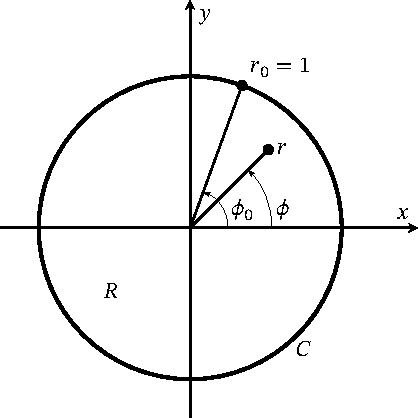
\includegraphics[width=0.7\linewidth]{sample-figure-1.pdf}
\caption{Figure caption with math, eqn.~\eqref{eqn:fourier}: $z = (r,\phi)$ \cite{Lienhard2019b}\label{fig:1}}
\end{figure}
 
%%%%%%%%%%%%% end figure %%%%%%%%%%%%%%%%%%%


%%%%%%%%%%%%%%%%%%%%%%%%%%%%%%%%%%%%%%%%%%%%%%%%%%%%%%%%%%%

%% Use title case for subsections and subsubsections

\section{Section Headings and Captions}
ASME requires that section headings and captions be set in an uppercase, sans serif font.  The class will do this automatically.  You can place \verb|\cite{..}|, \verb|\ref{..}|, \verb|\label{..}|, and mathematics into headings and captions directly, as you would in the main text. Do not enclose them braces, e.g.\ \verb|{\cite{..}}|, which will cause errors. You can place \verb|\footnote{..}| into headings, but not into captions.\footnote{See \texttt{tex-stackexchange} for various approaches to footnotes in captions, if they seem necessary. For footnotes in tables, use the \texttt{tablefootnote} package.}\footnote{Sequential footnotes are automatically separated by a comma.}

Text in section headings and captions will not be capitalized if enclosed in a \verb|\NoCaseChange{..}| command.

Sections may either be numbered or left unnumbered.

Simple mathematical expressions can be used in either captions or section headings. For a section heading that includes more complicated math (and macros), you may use the optional argument of \verb|\section[..]{..}| to create a pdf bookmark without losing characters or producing warnings or errors. See the \texttt{asmeconf-template.tex} source file for examples of this procedure. These bookmarks should usually be text expressions, although some math is supported.  

If you wish to override the default math format in captions, put \verb|\mathversion{normal}| in the caption.

\subsection{Subsection and Sub-subsection Headings}
Subsections and sub-subsection headings should be entered in title case, with the first letter of primary words capitalized. Sub-subsections (i.e., paragraphs) are never numbered.


%%%%%%%%%%%%%%% begin simple table %%%%%%%%%%%%%%%%%%%%%%%%%% 

%% captions go above tables

\begin{table}[t]
\caption[Table]{A simple table\label{tab:1}}
\centering{%
\begin{tabular}{l l r}
\toprule
Experiment & $u$ [m/s] & $T$ [\textdegree C] \\
\midrule
Run 11 & 12.5 & 103.4 \\
Run 12 & 24   & 68.3 \\
\bottomrule
\end{tabular}
}
\end{table}

%%%%%%%%%%%%%%%% end table  %%%%%%%%%%%%%%%%%%%%%%%%%%%%%%%%%%%% 

%%%%%%%%%%%%%%% begin more complicated table %%%%%%%%%%%%%%%%%%%%%%%%%%%%%%%%%%%%

\begin{table}[t]
\caption{Table with more complicated columns}\label{tab:2}%
\centering{%
\begin{tabular}{!{\hspace*{0.5cm}} >{\raggedright\hangindent=1em} p{3cm} d{3.3} @{\hspace*{1cm}} d{3.3} !{\hspace*{0.5cm}}}
\toprule
Experiment & \multicolumn{1}{c@{\hspace*{1cm}}}{$u$ [m/s]} & \multicolumn{1}{c!{\hspace*{0.5cm}}}{$T$ [\textdegree C]} \\
\midrule
The first test we ran this morning   & 124.3     &   68.3   \\
The second test we ran this morning  &  82.50    &  103.46  \\
Our competitor's test                &  72.321   &  141.384 \\
\bottomrule
\end{tabular}
}
\end{table}

%%%%%%%%%%%%%%%% end table  %%%%%%%%%%%%%%%%%%%%%%%%%%%%%%%%%%%% 

%%%%%%%%%%%%%%%%%%%%%%%%%%%%%%%%%%%%%%%
\section{Tables and Figures}

Table \ref{tab:1} is an example of a simple table. Table captions should be placed above tables.
The class loads the \texttt{booktabs} package (used for horizontal rules in both Table \ref{tab:1} and \ref{tab:2}), and the \texttt{array} and \texttt{dcolumn} packages which provide extended capabilities for columns in the \texttt{tabular} environment (used in Table \ref{tab:2}).  Table \ref{tab:3} is an example of a table that spans two columns. Two column tables (and figures) will always float to the top of a later page.

Figure captions go below figures. Figure~\ref{fig:2} is an example of a figure that spans two columns and includes subfigures. The text in figures (and tables) should be no smaller than 6~point type. Images in figures are handled by the standard \texttt{graphicx} package.

Landscape figures and tables may be produced at full-page size by putting \verb|\usepackage[figuresright]{rotating}| in your \texttt{.tex} file's preamble and using the \texttt{sidewaystable*} and \texttt{sidewaysfigure*} environments~\cite{fairbairns}.

%%%%%%%%%%%%%%% begin two column table %%%%%%%%%%%%%%%%%% 
\begin{table*}
\caption{A table spanning two columns\label{tab:3}}%
\centering{%
\begin{tabular*}{0.8\textwidth}{@{\hspace*{1.5em}}@{\extracolsep{\fill}}ccc!{\hspace*{3.em}}ccc@{\hspace*{1.5em}}}
\toprule
\multicolumn{1}{@{\hspace*{1.5em}}c}{$x$\rule{0pt}{11pt}} &
\multicolumn{1}{c}{$\textrm{erf}(x)$} &
\multicolumn{1}{c!{\hspace*{3.em}}}{$\textrm{erfc}(x)$} &
\multicolumn{1}{c}{$x$} &
\multicolumn{1}{c}{$\textrm{erf}(x)$} &
\multicolumn{1}{c@{\hspace*{1.5em}}}{$\textrm{erfc}(x)$} \\ \midrule
0.00 & 0.00000 & 1.00000 & 1.10 & 0.88021 & 0.11980\rule{0pt}{11pt} \\
0.05 & 0.05637 & 0.94363 & 1.20 & 0.91031 & 0.08969 \\
0.10 & 0.11246 & 0.88754 & 1.30 & 0.93401 & 0.06599 \\
0.15 & 0.16800 & 0.83200 & 1.40 & 0.95229 & 0.04771 \\
0.20 & 0.22270 & 0.77730 & 1.50 & 0.96611 & 0.03389 \\
0.30 & 0.32863 & 0.67137 & 1.60 & 0.97635 & 0.02365 \\
0.40 & 0.42839 & 0.57161 & 1.70 & 0.98379 & 0.01621 \\
0.50 & 0.52050 & 0.47950 & 1.80 & 0.98909 & 0.01091 \\
0.60 & 0.60386 & 0.39614 & 1.82\makebox[0pt][l]{14} & 0.99000 & 0.01000 \\
0.70 & 0.67780 & 0.32220 & 1.90 & 0.99279 & 0.00721 \\
0.80 & 0.74210 & 0.25790 & 2.00 & 0.99532 & 0.00468 \\
0.90 & 0.79691 & 0.20309 & 2.50 & 0.99959 & 0.00041 \\
1.00 & 0.84270 & 0.15730 & 3.00 & 0.99998 & 0.00002 \\[2pt]
\bottomrule\end{tabular*}
}
\end{table*}

%%%%%%%%%%%%%%%%% end two column table  %%%%%%%%%%%%%%%%%%%%%%%%%%%%%%% 




%%%%%%%%%%%%%%%%%%%%%%%%%%%%%%%%%%%%%%%%%%%%%%%%%%%%%%%%%%%%%%%%%%%%%%

\section{Reference Formatting with \NoCaseChange{\texttt{asmeconf.bst}}\footnote{If you have text in a section heading or caption that you do not want to be capitalized, such as an SI unit, enclose it in a \texttt{\textbackslash NoCaseChange} command.}}\label{sec:references}

The {\upshape\texttt{asmeconf.bst}} \hologo{BibTeX}  style follows the reference styles shown on ASME's conference web site in early 2020. Examples for these and many other cases are given in the \texttt{asmeconf-sample.bib} file, which is part of this distribution. Citations and references are managed by the standard \texttt{natbib} package.  Nevertheless, a few comments are necessary. 

%% sub-subsections should *not* be numbered

\subsubsection*{DOI, URL, and eprint} Include DOI numbers when they are available.  URL's may alternatively be given. ASME requests that URLs point to a document's abstract.

Elementary support for \texttt{eprint} numbers is also included, generating a url at the end of the citation. The \texttt{archive} type may be specified using the macros \texttt{arxiv, googlebooks, hdl, jstore, oclc}, or \texttt{pubmed} (e.g., \texttt{archive=hdl},  \textit{without} braces). Both \texttt{eprint} and \texttt{archive} fields \textit{must} be given. Other root urls may be invoked using \verb|archive = {http://another.url.org/}|.

\subsubsection*{Online Sources} A bibliography field \verb|@online{..| is included for citation of online sources, such as web pages. A \texttt{url} or \texttt{eprint} with \texttt{archive} must be included. See the examples of use in the \texttt{asmeconf-sample.bib} file. 

\subsubsection*{Date Accessed} The \verb|urldate={..}| field may be used to provide the date on which a given url was accessed. By default, the text printed will be \texttt{Accessed `date',}. The word ``Accessed'' may be changed using the \verb|urltype={..}| field.

\subsubsection*{Conference Location and Date} For the entry types \verb|@inproceeedings{..| and \verb|@proceeedings{..|, you may include \verb|venue={..}| and \verb|eventdate={..}| to specify the city and the date of a conference.

\subsubsection*{Capitalization of Titles} ASME's bibliography style requires that document titles be in title case. The first letters of principal words are capitalized. Do this when writing the \texttt{.bib} file.



%%%%%%%%%%%%%%%%%  begin two column figure  %%%%%%%%%%%%%%%%%%%%%%%%%%%

\begin{figure*}
\begin{subfigure}[t]{0.5\textwidth} %subfigure is basically the same as minipage
\vbox{
\vspace*{1.7em}
\centering{
  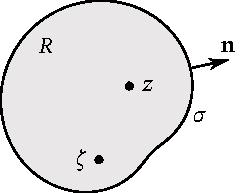
\includegraphics{sample-figure-2a.pdf}
}
\vspace*{1.7em}
}
\subcaption{Interior region\label{fig:interior-region}}
\end{subfigure}%
%%%%%%%%%%%%% no spaces or line breaks between these two subfigures
\begin{subfigure}[t]{0.5\textwidth}
\centering{%
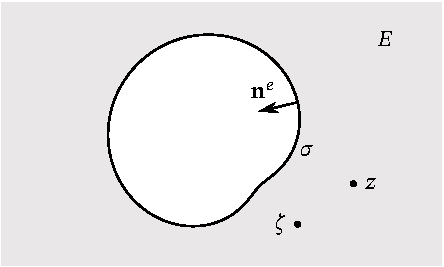
\includegraphics{sample-figure-2b.pdf}
\subcaption{Exterior region\label{fig:exterior-region}}
}\end{subfigure}
\caption{A figure with two subfigures  \cite{Lienhard2019b}}\label{fig:2}
\end{figure*}

%%%%%%%%%%%%%%%%%%%  end two column figure  %%%%%%%%%%%%%%%%%%%%%%%%%%


%%%%%%%%%%%%%%%  MORE ON MATH   %%%%%%%%%%%%%%%%%%%%%%%%%%%%%%%%%%%%%%%%%%%%%%%%%%%%%%%%%%%%%%%%%%%%%%

%% Dealing with complicated math in a section or subsection heading: 
%%    the optional argument to \section will provide the pdf bookmark
%%    without losing characters or producing warnings/errors.
%%
%% In this heading, letter u is forced to be upright with \mathrm{u}
%%
\section[More on math: u\cdot\omega=0]{More on math: $\vec{\mathrm{u}}\cdot\vec{\omega}=0$}\label{sec:moremath}

In most cases, the need for a wide equation can be eliminated by using one of the multiline equation environments defined by 
\texttt{amsmath}, such as \texttt{align}, \texttt{split}, or \texttt{multline}~\cite{amsmath}. The following equation is set with the 
\texttt{multline} environment:
\begin{multline}\label{eqn:energy}
\frac{\partial}{\partial t}\left[\rho\bigl(e + \lvert\vec{u}\rvert^2\big/2\bigr)\right]  + \nabla\cdot\left[\rho\bigl(h + \lvert\vec{u}\rvert^2\big/2 \bigr)\vec{u}\right] \\
 ={}-\nabla \cdot \vec{q} +  \rho \vec{u}\cdot\vec{g}+ \frac{\partial}{\partial x_j}\bigl(d_{ji}u_i\bigr) + \dot{Q}_v
\end{multline}
An example using \texttt{align} appears in Appendix~\ref{appendix:a}.

An alternative solution may be to set large equations into two-column-wide tables or figures. While a package exists for setting equations that span two columns (\texttt{widetext.sty}), that code is erratic in relation to floats and page breaks.

Math italics are used for roman and greek letters by default.  If you want an upright letter in math, you can use the relevant math alphabet, e.g., \verb|\mathrm, \mathbf, \mathsf|:
\begin{equation}\label{eqn:dw}
\vec{F} = m \vec{a} \quad\textrm{or}\quad \vec{\mathrm{F}} = m \vec{\mathrm{a}} \quad\textrm{or}\quad \mathbf{F} = m \mathbf{a} \quad\textrm{or}\quad \vec{\mathsf{F}} = m \vec{\mathsf{a}}
\end{equation}
To get additional symbols in bold math, you can use the \verb|\bm{..}| macro from the \texttt{bm} package, which is loaded by the class.

The class file also provides upright sans-serif greek letters with \verb|\sfalpha| and similar expressions (e.g., $\sfalpha, \sfbeta, \sfgamma, \sfdelta$ \ldots $\bm{\sfalpha, \sfbeta, \sfgamma, \sfdelta \ldots}$), in case they are needed (but note that the \verb|newtxmath| options \verb|frenchmath| and \verb|slantedGreek| also affect how greek letters are presented).

\subsection{The \texttt{newtxmath} and \texttt{mathalpha} Packages~\cite{sharpe1,sharpe2}} The \texttt{newtxmath} package~\cite{sharpe1}, loaded by default, includes a large number of options for mathematics, most of which can be called as options to \verb|\documentclass|. For example, the \texttt{upint} option of \texttt{newtxmath} selects upright integral signs (rather than slanted integral signs):
\begin{quote}
\verb|\documentclass[upint]{asmeconf}|. 
\end{quote}  
These math options are discussed further in the \texttt{asmejour-template.tex} file. 

In addition, many options for calligraphic, fraktur, and script fonts are available as options to the \texttt{mathalfa} package, which is also loaded. These may be invoked, for example, as 
\begin{center}
\verb|\documentclass[mathalfa=cal=euler]{asmeconf}| 
\end{center}
which selects the Euler font for \verb|\mathcal| (this is our default). To find all the font options, refer to the \texttt{mathalfa} package documentation \cite{sharpe2}.

The typewriter font loaded is \texttt{inconsolata} (which is sans serif), as suggested by the \texttt{newtx} package documentation. 

The \texttt{asmeconf} class is not set up for use with the \texttt{fontspec} or \texttt{unicode-math} packages.


%%%%%%%%%%%%%%%  ADDITIONAL PACKAGE OPTIONS  %%%%%%%%%%%%%%%%%%%%%%%%%%%%%%%%%%%%%%%%%%%%%%%%%%%%%%

\section{Additional Options for \NoCaseChange{\texttt{asmeconf.cls}}}
The class accepts a number of options in addition to those already described. These options are discussed next.

\subsection{Colored hyperlinks}
ASME requires that all text be \textbf{in black} when the paper is submitted for publication.  For other uses, authors may
obtain colored hyperlinks with the [\texttt{colorlinks}] option.

\subsection{Final Column Balancing} The option \texttt{[balance]} invokes the the \texttt{flushend} package~\cite{tolusis}.
This package will attempt to give equal height to the two columns on the last page. The performance of this package is sometimes inconsistent (with odd page layout or, very rarely, errors), so use this option with caution.

\subsection{Line Numbers} The option \texttt{[lineno]} invokes the the \texttt{lineno} package~\cite{bottcher}. This option will produce line numbers in the margins. You must run \LaTeX\ \textit{twice} for proper placement of the numbers. Tables, captions, and footnotes will not be numbered.  Line numbers can be helpful for review and editing, but should not be used in your final manuscript. See the documentation of the \texttt{lineno} package for further commands to control line numbering. 

The \texttt{lineno} package is not compatible with the \texttt{flushend} package that makes final short columns the same height. Balancing is automatically disabled when this option is called. 

\subsection{Changing the Footer Text} The option \texttt{[nofoot]} will omit the ASME copyright from the first page footer. 
The footers are generated with the \texttt{fancyhdr} package~\cite{oostrum}, so you can change them in any way you like using the commands of that package. Only the default arrangement of footers matches ASME's style, however.

\subsection{Superiors Font} The \texttt{newtxtext} package includes a superiors font (both numbers and letters) for use in footnote markers and superscripts. To enable this font, use the option \texttt{[nodefaultsups]}. 

\subsection{Old-style Author Grid} The option \texttt{[oldauthors]} invokes ASME's old grid-style arrangement of author names.  The authors and affiliations must be entered differently in this case. See Appendix \ref{appendix:b} for usage.

\subsection{Hyphenation of Typewriter Font} The option \texttt{[hyphenate]} will allow hyphenation of the typewriter font.
Hyphenation is normally suppressed for typewriter mode because this font is often used for code.

\subsection{Support for Other Languages}  The package can be adapted to incorporate (or entirely use) languages other than English. See Appendix \ref{appendix:c} for details.

%%%%% Conclusions %%%%%%%%%%%%%%%%%%%%%%%%%%%%%%%

\section{Conclusion}
Provide a brief conclusion (3-4 lines).


%%%%% Acknowledgments %%%%%%%%%%%%%%%%%%%%%%%%%%%

\section*{Acknowledgments}
Place any acknowledgments here.



%%%  REFERENCES  %%%%%%%%%%%%%%%%%%%%%%%%%%%%%%%%
%%
%% Put your references into your .bib file in the usual way. Run latex once, bibtex once, then latex twice.
%% The asmeconf.bst style allows: venue = {Location of Conference}, and eventdate = {Month, days}
%%		for @inproceedings and @proceedings
%%

\nocite{*} %% <=== Delete this line unless you want to typeset the entire contents of your .bib file!

\bibliographystyle{asmeconf}   %% .bst file following ASME conference format. Do not change.
\bibliography{asmeconf-sample} %% <=== change this to name of your bib file


%%%  APPENDICES  %%%%%%%%%%%%%%%%%%%%%%%%%%%%%%%%
\appendix

%% Note that appendices will be "numbered" A, B, C, ... etc. Use \section, not \section*
%% Equations will be numbered sequentially following those in the paper. Do not reset the equation counter.

%% Here we use the optional argument for the pdf bookmark.
\section[The vector product A\times B]{The vector product $\vec{A}\times\vec{B}$}\label{appendix:a}

This brief illustration of an appendix shows the numbering of the appendix and equations. Equations are numbered
consecutively, following those in the paper.
\begin{align}
\frac{d\Gamma}{dt}   &{}= \int_{\mathcal{C}} \frac{D\mathbf{u}}{Dt} \cdot d\mathbf{r}\\
                                  &{}= \iint_{\mathcal{S}} \nabla \times \frac{D\mathbf{u}}{Dt}  \cdot d\mathbf{A}\\
                                  &{}= \iint_{\mathcal{S}}  \nabla p \times \nabla \left( \frac{1}{\rho}\right) \cdot d\mathbf{A}
\end{align}


\section{Option to use an author grid}\label{appendix:b}

ASME's most recent templates place author names inline, with affiliations for all authors in rows below. 
This style is the default for this template.  

The historical style of authors with affiliation in a grid of blocks may be invoked with
the option [\texttt{oldauthors}].  When using this form, the author names and addresses should be entered as below:

\smallskip
\noindent\verb|\SetAuthorBlock{Name\JointFirstAuthor}{%|
 \hbox{}\hfil\verb|Institution \\ City, State}| 
\verb|\SetAuthorBlock{Name\JointFirstAuthor}{%|
 \hbox{}\hfil\verb|Institution \\ City, Country}|
\verb|\SetAuthorBlock{Name, Name}{%|\hfil\hbox{}
 \noindent\hbox{}\hfil\verb|Institution \\ City, Country}|
\verb|\SetAuthorBlock{\CorrespondingAuthor{John Lienhard%|
 \hbox{}\hfil\verb|}{lienhard@mit.edu}}{Institution \\ City, State}|
 
Directly usable code is contained at the very end of the \texttt{asmeconf-template.tex} file.

%% directly usable code follows the \end{document} command below.


%%%%%%%%%%%%%%%%%%%%%%%%%%%%%%%%%%%%%%%%%%%%%%%%%%%%%%%%%%%%%%%%%%%%%%
\section{Language Support}\label{appendix:c}

ASME publishes in English, but the \texttt{babel} package is loaded for 
users who may wish to include other languages. Options are supported to load a primary language, \texttt{lang=}, 
as well as a secondary and tertiary language, \texttt{lang-second} and \texttt{lang-third}.  
The primary language must be specified explicitly if a secondary language is loaded.  
If no language option is given, the package defaults to English.  An example of use is 
shown in \selectlanguage{french}\appendixname\ \ref{app:fourier}.\selectlanguage{english}

The standard caption and section names will follow \texttt{babel}'s dictionary for primary languages other than English.  Users may additionally change ``Keywords'', ``Nomenclature'',  ``Corresponding author'', and ``Joint first authors'' by renewing the commands \verb|\keywordname|, \verb|\nomname|, \verb|\CAwords|, and \verb|\JAwords|. Changes to the page footer were described earlier. The pdf bookmark for ``Appendices'' may be changed by renewing \verb|\appendicesname|.

Font encoding is set to T1 with utf-8 input supported: 
%% If you have trouble with the next line, your file may not be saved in utf-8 format. You can delete that line to resolve the issue.
\typeout{If you have trouble with the next line, your file may not be saved in utf-8 format. You can delete that line to resolve the issue.}
àáâäæãåā  èéęëêēė  îïíīįì ôöòóœøōõ ûüùúū çćč ł ñń ßśš ÿ žźż.

No effort has been made to support customization of language-specific fonts, although this is possible by modifying the class file (examples are given in the \texttt{newtx} documentation). The bibliography style, \texttt{asmeconf.bst}, is designed in English and aimed at \hologo{BibTeX}.  Multilingual bibliographies can be supported using \texttt{BibLaTeX}.

\selectlanguage{french}
\section{Discours Préliminaire de Fourier}\label{app:fourier}

Les causes primordiales ne nous sont point con­nues; mais elles sont assujetties à des lois simples et constantes, que l'on peut découvrir par l'obser­vation, et dont l'étude est l'objet de la philosophie naturelle. 

La chale ur pénètre, comme la gravité, toutes les substances de l'univers, ses rayons occupent toutes les parties de l'espace. Le but de notre ouvrage est d'exposer les lois mathématiques que suit cet élé­ment. Cette théorie formera désormais une des branches les plus importantes de la physique gé­nérale~\cite{fourier1822}. 

\selectlanguage{english} 

\end{document}


%%% This is the set-up for the old author block style, a grid of blocks.

% Can also put multiple emails and use command more than once for multiple corresponding authors.
% Change to your name[s] and addresses, in the desired order of authors. Up to nine author blocks.
% Note usage below for joint first authors and for corresponding author.
% First name, middle initial, last name
% Use title case (upper and lower case letters)
%    (Most of the example names below are not real people, just very common names.)

\SetAuthorBlock{Luis Hern\'{a}ndez\JointFirstAuthor}{Institution or Company Name, City, State} 
\SetAuthorBlock{Maria Silva\JointFirstAuthor}{Institution or Company Name, City, Province, Canada}

\SetAuthorBlock{Henry Tudor,  Catherine Parr}{Hampton Court Palace \\ Richmond, England}
\SetAuthorBlock{Jinsoo Kim}{Institution or Company Name, City, Country}
\SetAuthorBlock{Yusuf Yilmaz}{Institution or Company Name, City, Country}

% Can omit second argument of \CorrespondingAuthor if putting email into address
%   i.e., can just use \CorrespondingAuthor{name}. 
% Can also put multiple emails in the command and use more than once for multiple corresponding authors.

\SetAuthorBlock{\CorrespondingAuthor{John H.\ Lienhard V}{lienhard@mit.edu}}{%
Massachusetts Institute of Technology \\  Cambridge, MA}


